\begin{frame}{Vertival error of $d(K^-, n)"\pi^{\mp}\Sigma^{\pm}"$}
  \small
  \begin{itemize}
  \item $d(K^-, n \pi^+ \pi^-)"n"$の統計エラー $\sim 3.9\%$
  \item $d(K^-, n \pi^+)"\Sigma^-"$ and $d(K^-, n \pi^-)"\Sigma^+"$のフィッティングの系統エラー\\
    $d(K^-, n \pi^-)"\Sigma^+" \sim 4.8\%$ $d(K^-, n \pi^+)"\Sigma^-" \sim 8.6\%$ average$\sim 4.4\%$ \\
    \hspace{6.5cm} (各最大値に対する割合)
  \item カウント数$\rightarrow$断面積のファクターの系統エラー $\sim 5.6\%$
  \item 全エラーの自乗平均平方根/最大値\\
    $d(K^-, n \pi^-)"\Sigma^+" \sim 8.4\%$ $d(K^-, n \pi^+)"\Sigma^-" \sim 10.0\%$ average$\sim 8.1\%$ \\
  \end{itemize}
  \begin{tabular}{cc}
    \begin{minipage}{0.5\hsize}
      \begin{figure}
        \centering
        \footnotesize
        $d(K^-, n)"\pi^{\mp}\Sigma^{\pm}"$
        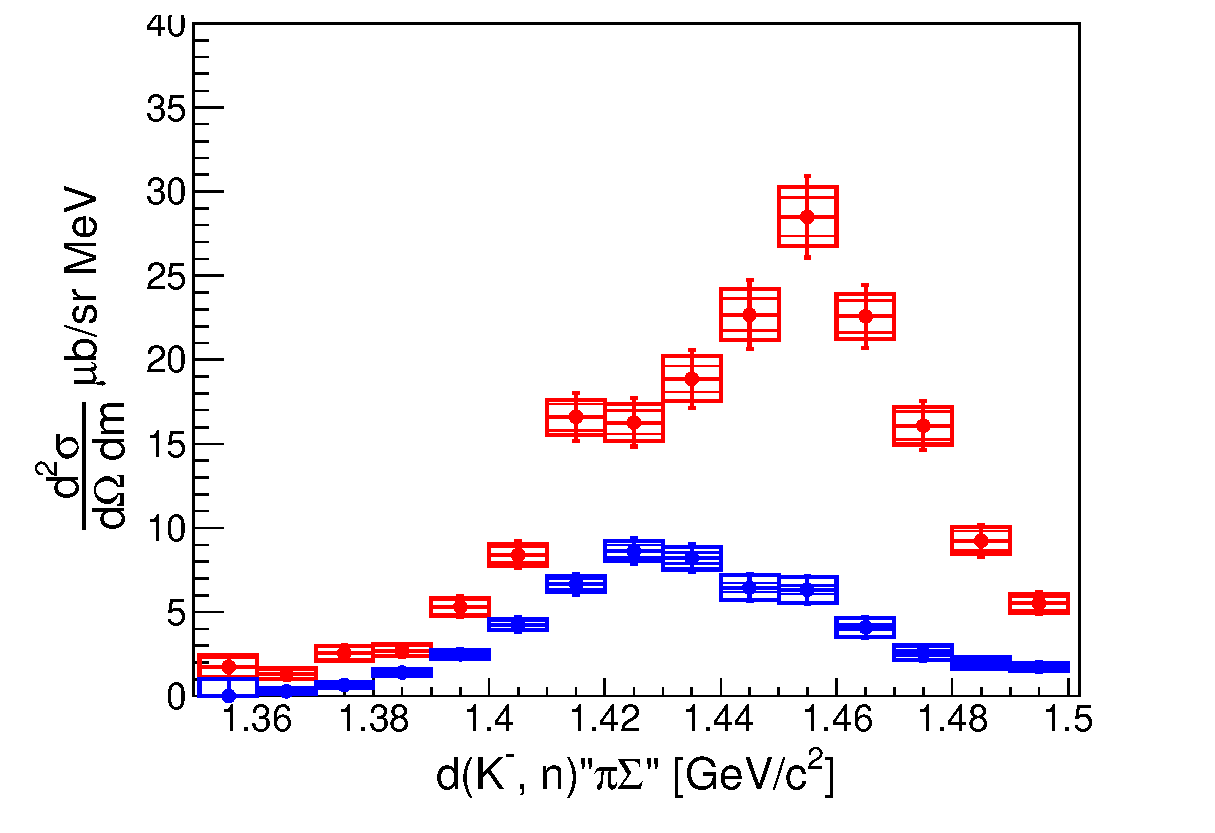
\includegraphics[width=5cm]{../pic/Run78/K0_ts_L1520/ChargeCS_after.eps}
      \end{figure}
    \end{minipage}
    \begin{minipage}{0.5\hsize}
      \begin{figure}
        \centering
        \footnotesize
        Average CS\\
        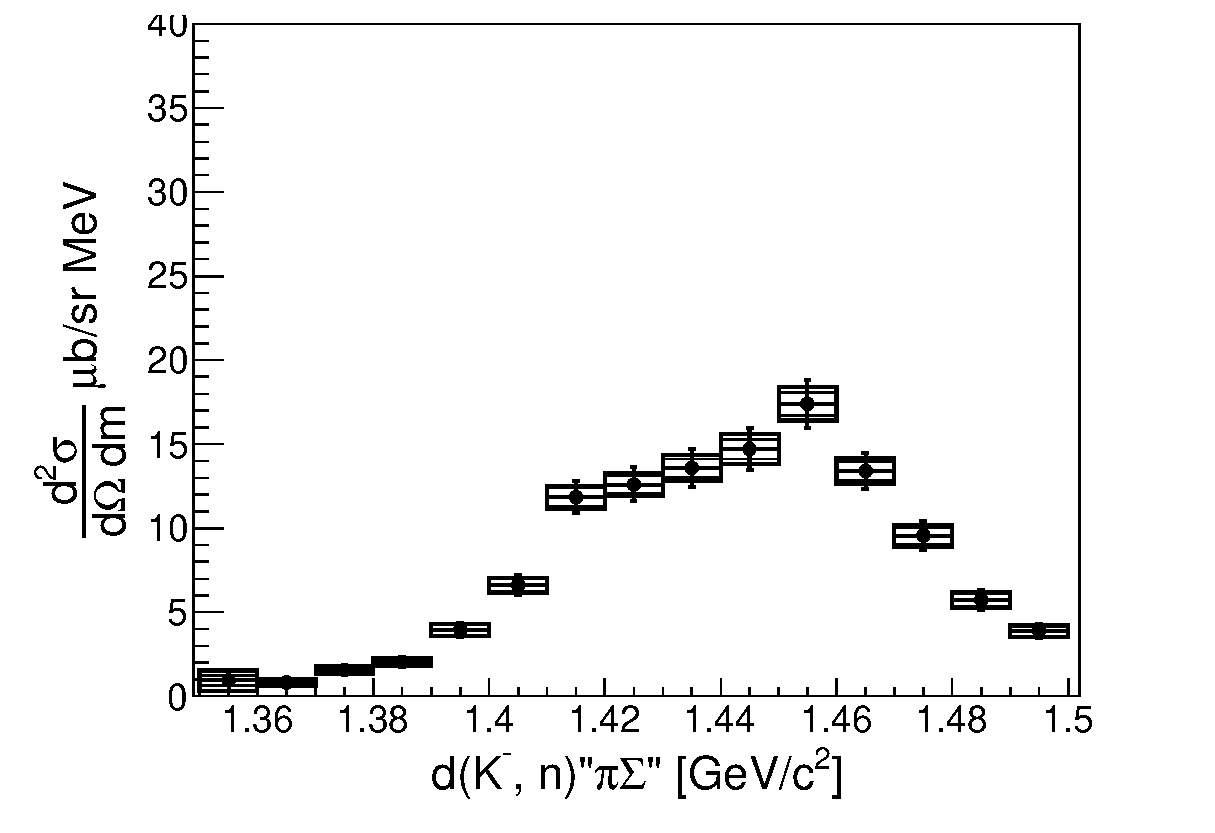
\includegraphics[width=5cm]{../pic/Run78/K0_ts_L1520/ChargeCS_ave_after.eps}
      \end{figure}
    \end{minipage}
  \end{tabular}
\end{frame}
